% This chapter with be all the B2 stuff as well as the introduction and definiton of the project

\chapter{Project Definition} % Main chapter title
\label{Chapter1} % Change X to a consecutive number; for referencing this chapter elsewhere, use \ref{ChapterX}

%----------------------------------------------------------------------------------------
%	SECTION 1
%----------------------------------------------------------------------------------------
\tocdata{toc}{Edward Gunn}
\section{Introduction}
\sectionmark{Introduction - Edward Gunn}
The process of writing music often begins with an idea for a melody which is followed by the development of chords to accompany it.
The matching of chords to a melody is a skill which usually requires years of training in musical techniques such as harmonisation.
There is a large market of amateur musicians who lack the necessary training for this task but would otherwise enjoy the experience of developing music.  
In this report we will detail the design of ReChorder, a system which facilitates the generation of an appropriately matched set of chords to a given monophonic melody.
Users are able to record a melody using their microphone and regenerate the chord sequence until they feel they have found one suitable for the intended feel of their song.
Songs and generated chord accompaniments can be played back to the user, saved to a library of songs and shared using our songwriting community feature. \\
The problem of converting a recorded melody to a set of chords can be decomposed into a set of simpler sub-problems, these being:
the conversion of the recorded melody into a form which numerically represents its features,
and the generation of a set of chords from this numerical representation.
The latter of these two problems can be solved in a variety of ways, many of which require a detailed knowledge of music to find patterns in melodies to match to chords.  
%\textbf{WHY IS THIS A PROBLEM FOR US}
A method which requires little knowledge of music is the use of a machine learning model to extract these patterns from data of known chord melody pairings from professionally composed music. 
The curation and processing of an appropriate dataset requires significant effort and care in itself.
This leads to a natural division of labour across the project into the categories of:\label{sec:Introduction}
User Interface and general product design - detailed in \cref{Chapter2} by Di Wan;
recommendation engines for our community feature - detailed in \cref{Chapter6} by Di Wan;
the conversion of recorded melody to the same format as expressed in the dataset - detailed in \cref{Chapter5} by Kitty Fung;
curation and preparation of a dataset in an appropriate format - detailed in \cref{Chapter3} by Terence Tan;
the design of an appropriate machine learning model - detailed in \cref{Chapter4} by Edward Gunn.



%-----------------------------------
%	SUBSECTION 1
%-----------------------------------
\subsection{Musical terminology}
Throughout this report we will use a variety of musical terminology which will be defined here. A piece of music is composed of a sequence of adjacent \textbf{measures}, periods of time in which notes and chords can be played. 
We will generally take a \textbf{measure} to mean a bar in the music, however it is not restricted to this. We restrict \textbf{chord} to refer to a triad of notes. %, the justification for this is explained in \textbf{reference to explanation}.
The use of \textbf{melody} refers to a monophonic melody in which only one note is played at a time, excluding accompanying chords, unless otherwise stated.
\textbf{Tempo} will refer to the speed of the music usually measured in beats per minute or bpm.
\textbf{Time Signature} refers to an integer pair specifying in the top element the number of beats in a bar and in the bottom element the length of note which will represent a beat.
\textbf{Timbre} is defined as the perceived sound quality of a tone and is affected by its overtones.
%-----------------------------------
%	SUBSECTION 2
%-----------------------------------

\subsection{Project Overview}
\label{Project Overview}
\begin{figure}
    \centering
    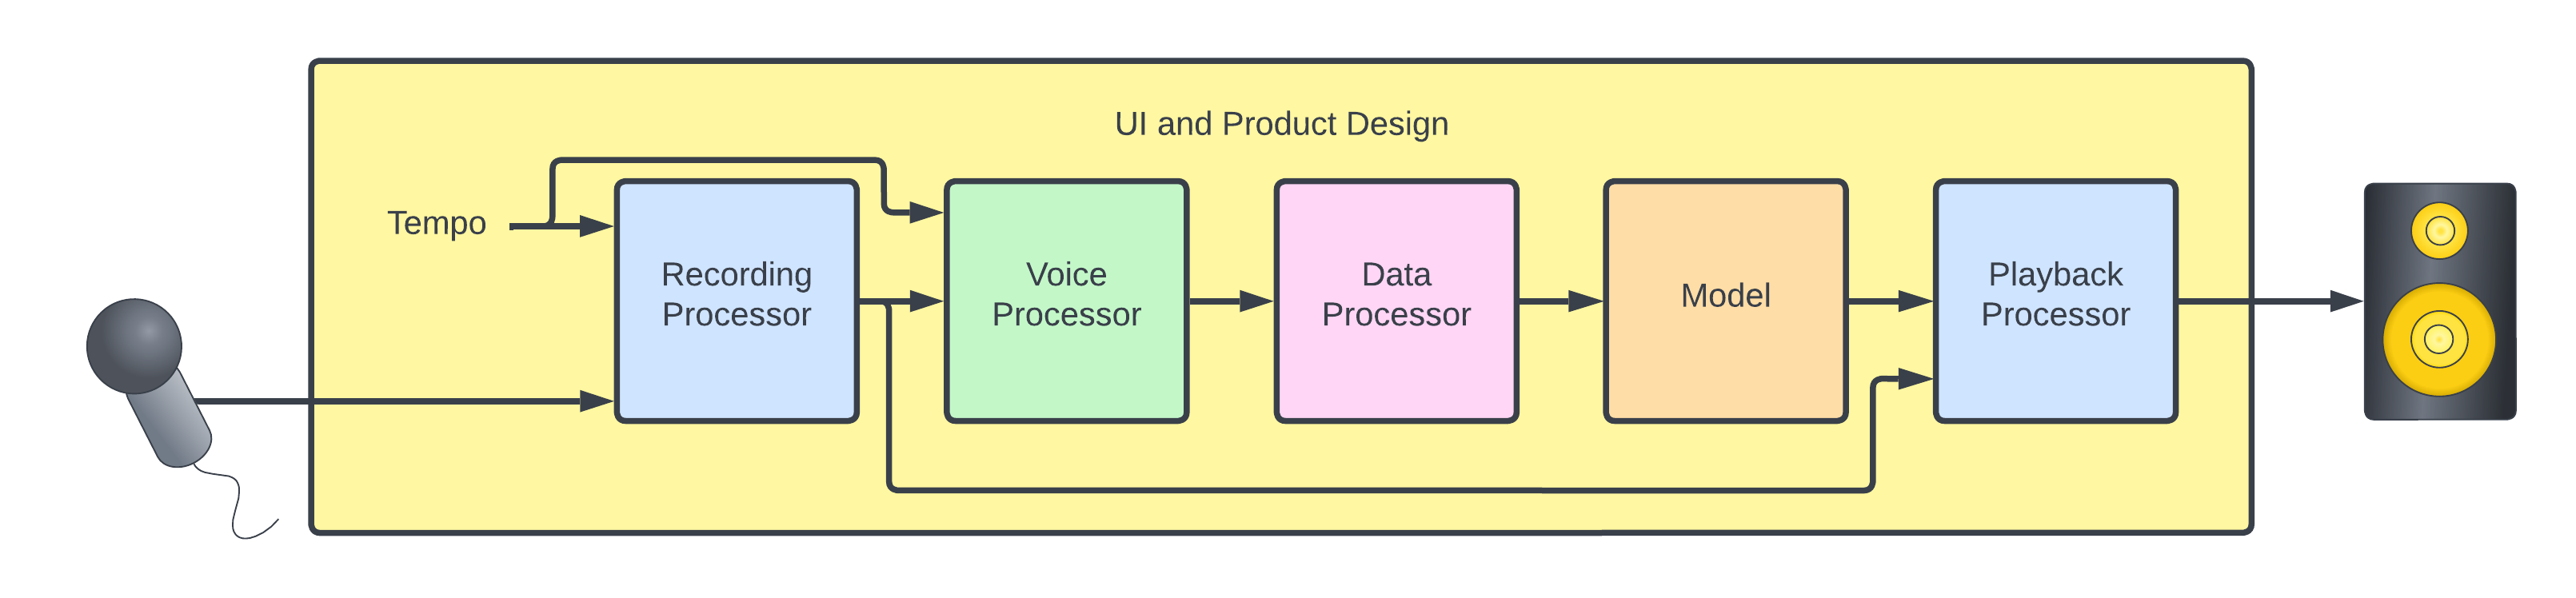
\includegraphics[width=0.8\columnwidth]{Figures/Project Overview}
    \decoRule
    \caption[]{An overview of the internal workings of ReChorder}
    \label{fig:MVPOverview}
\end{figure}

\paragraph{Overview}
To achieve the goal of this project, the product design should be capable of producing chords which appropriately accompany a monophonic melody, allowing amateur musicians to compose music quickly and easily.
As seen in \cref{sec:Introduction} this problem can modularised into a number of independent parts, each solving a sub-problem, which when connected end to end can solve the problem as a whole.
A minimum viable product (MVP) was defined to specify ReChorder's essential functionality.
The MVP is further detailed in \cref{sec:UImvp} and \cref{sec:MVPRequirements}.
For the MVP the required modules are as follows: the Recording Processor, the Audio Pre-processor, the Data Processor, the Model, the Playback Processor.
In the desired final product these are accessed through a purpose built user interface.

\paragraph{Recording Processor}

The function of the recording processor is to allow the user to specify a given time signature and tempo and record a melody to be passed to the voice processor.
When the recording is started a digital metronome can be played to guide the user's tempo. 
Although not necessary in the MVP a feature of the recording processor could be added such that if the metronome is used its influence on the recording is subtracted thus giving a clearer recording at a consistent tempo.
Using a high quality setup for recording this problem could potentially be solved by simply subtracting the know waveform of the metronome from the waveform of the recording, but this is an area for future work.
Once the recording is complete it is passed to the Voice Processor along with the time signature and tempo of the piece.

\paragraph{Audio Pre-processor}

The function of the audio pre-processor is to extract the musical features present in our Model's training dataset from a noisy recording of the user's melody and put these in the same form as the raw dataset.
This processing involves three main steps: filtering, pitch detection and key detection.
The recoding must first be filtered to remove noise, then the pitch detection algorithm is used.
For each submeasure, using the time signature and tempo, the note played is determined giving for each song the notes that are played, which measure they are in and a rough estimate of the duration for which they are played.
The final step is to use the key detection algorithm to determine the key in which the piece is played.
The data is then passed to the data processor in the same form as the dataset for further processing.

\paragraph{Data Processor}

The function of the data processor is to convert the data into a format which can be used to train the model or used as input in production.
In training, we encode both the melody and chord data, putting it into vector format which can be inputted into the model, so the loss can be calculated by comparing the generated chords to the true chords.
In production, we encode the melody data, so it can be inputted into the model to generate chords.

\paragraph{Model}

The function of the model is fundamentally that of a sequence translator, translating from a sequence of melody vectors to a sequence of chord vectors.
We make use of machine learning to achieve this. 
The model is trained using the dataset to imitate real chord sequences which in production can be used to produce accompaniment for the input melodies.
The model passes its output to the playback processor.

\paragraph{Playback Processor}

The playback processor takes as input the output chords from the model and the recorded melody and plays these together, allowing the user to hear their generated accompaniment.
\tocdata{toc}{Edward Gunn}
\section{Software Design}
\sectionmark{Software Design - Edward Gunn}

The design for the software to implement each part of the project is heavily modularised, in keeping with the philosophies of object-oriented programming. 
We define self-contained objects that are composed of data and methods.
These objects each themselves utilise the ideas of encapsulation where objects act as a black box to other objects, composition where objects contain other objects, inheritance where a hierarchy of objects is created, a child object can inherit properties from its parent, and polymorphism where calling code is independent of where in a hierarchy an object is positioned.
In our product we defined an abstract template class for each module in order to maintain the interface upon implementation through inheritance.
The main ReChorder class is composed of an instance of each of the models where their implementation is irrelevant.
This allows us to easily swap out modules, for example, to test a different model.
The main functions for the app are concentrated in the ReChorder class.
These functions could be called directly from the user interface.
A UML diagram outlining the design can be seen in \cref{fig:SoftwareOverview}.


\begin{figure}
    \centering
    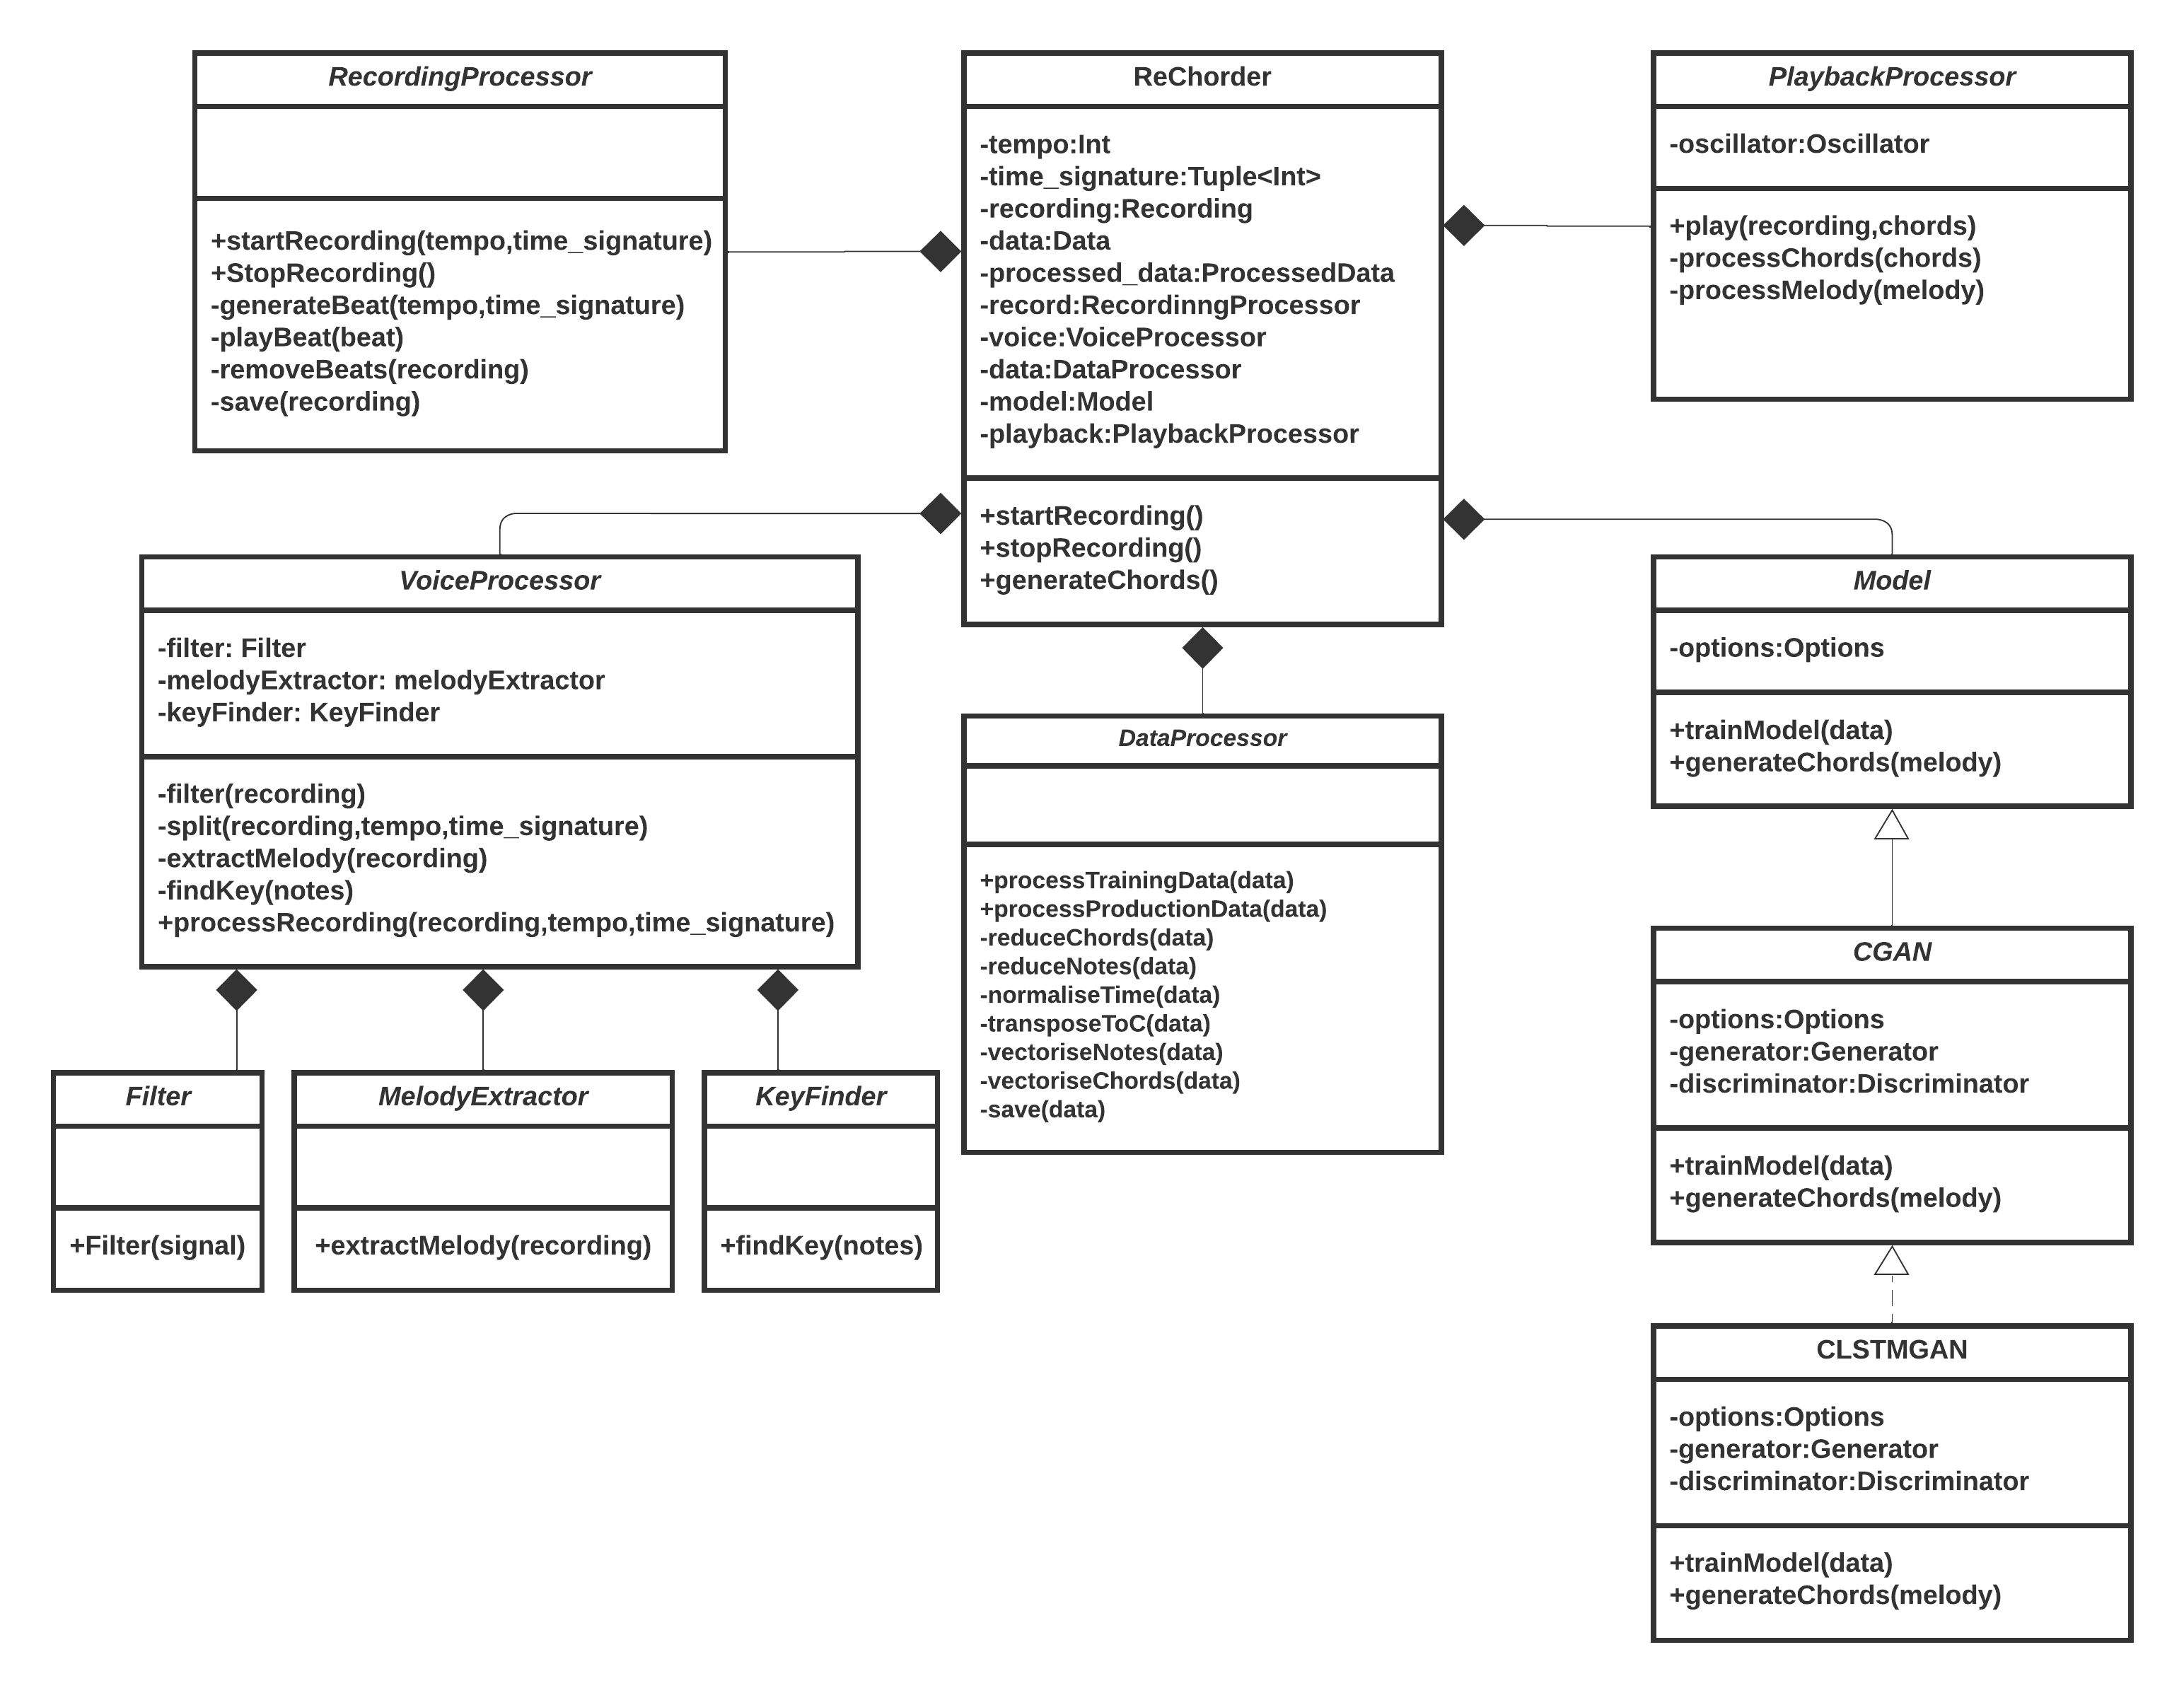
\includegraphics[width=\columnwidth]{Figures/SoftwareOverview}
    \decoRule
    \caption[]{An overview of the software design of ReChorder}
    \label{fig:SoftwareOverview}
\end{figure}

\tocdata{toc}{Terence Tan}
\section{Market Research}
\sectionmark{Market Research - Terence Tan}
\label{marketresearch}
As mentioned in the first few lines of \cref{sec:Introduction}, our product is aimed at amateur musicians. Research into our target demographic shows promising statistics. In the United Kingdom, the percentage of children who know how to play a musical instrument increased from 45\% in 1993 to 76\% in 2014, with 21\% of these children having never had lessons (\cite{abrsm2014}). Furthermore, 34\% of young people in the UK in 2021 create music on their own (\cite{abrsm2021}). In the United States, 22\% of people surveyed who play a music instrument said that they were self-taught (\cite{gallup2003}). Hence, it can be concluded that a significant proportion of musicians lack formal musical training, and that they have an interest in making music. In fact, self-taught musicians are more likely to create their own music (\cite{compareguitarpiano}). Additionally, 20\% of children in the UK have created music using a smartphone or tablet in 2014 (\cite{abrsm2014}), with 15\% of young people doing the same in 2021 (\cite{abrsm2021}). This implies that musicians would be receptive to creating music with digital applications. More importantly, given the time gap of seven years, the previous two statistics would be covering the same generation (many of the same children in 2014 would be youths in 2021). Yet, the numbers only decreased slightly from 20\% to 15\%. This is encouraging since it shows a sustained interest in creating music via digital means, which translates to a more stable and permanent consumer base for any digital music creation applications. Indeed, the percentage of adults who create music digitally barely dropped from 14\% in 2014 to 13\% in 2021 (\cite{abrsm2021}).
 
There is also evidence that self-taught musicians teach themselves through digital tools as well as peer-to-peer networks (\cite{abrsm2014})(\cite{bookreview}). There also seems to be a strong interest in creating and playing music with peers, with 40\% of children in the UK in 2014 creating music with friends outside of school (\cite{abrsm2014}). Self-taught musicians often play with other more experienced and better musicians to improve themselves in the process by learning from them (\cite{marketresearch5}). Thus, it seems that self-taught musicians would be interested in having access to a community of like-minded peers. 
 
Moreover, a YouGov survey (\cite{YouGovMR}) shows that 42\% of musicians professed to be singers, with more than half being self-taught. Guitar was the second most popular instrument behind piano, and 74\% of people who play the guitar said they were self-taught. This justifies the focus on converting singing to guitar chords for amateur musicians, since there is a substantial number of singers and guitar players who are self-taught.  

Given these findings, we can identify two main needs of our target market that our product can aim to meet. Firstly, our product has to be able to take vocals as inputs, and generate chords to accompany the singing. Secondly, our product has to provide a platform for a community of musicians that fosters collaboration and creativity. These two needs will be taken into account when designing our Minimum Viable Product (MVP) in \cref{sec:UImvp}.

%\subsection{Core functionalities of product}
%\label{coreproduct}

%Given the findings in Chapter \ref{marketresearch}, we can identify two main needs of our target market that our product can aim to meet. Firstly, our product has to be able to take vocals as inputs, and generate chords to accompany the singing. Secondly, our product has to provide a platform for a community of musicians that fosters collaboration and creativity.
%----------------------------------------------------------------------------------------
%	SECTION 2
%----------------------------------------------------------------------------------------
\tocdata{toc}{Edward Gunn}
\section{Project management}
\sectionmark{Project management - Edward Gunn}
\label{sec:Project management}
The project was conducted with an agile approach allowing us to quickly adjust to changes in the product as we learned and identified areas to improve on.
Agile works best in small teams with effective communication, and requires less formal training than traditional methods (\cite{Agile}) thus it was very well suited to our project. 
At the beginning of the project we clearly defined our objectives and wrote an MVP specification of a product we hoped to produce as proof of concept.
As stated in the introduction \cref{sec:Introduction} we divided the work into four distinct sections suited to the skills and experience each team member possessed and was interested in expanding.
Using the defined objectives and division of responsibilities we produced and prioritised a backlog of work to be completed, and created a timeline for this work to be completed in the form of a Gantt chart.
We organised week long sprints with a meeting at the end of each sprint to track our progress and adjust pace on lessons learned. 
Any work not completed in one sprint was carried over to the next.
A cadence of completing one piece of work each from the backlog per sprint was established.
Minutes were taken in the weekly meetings to record important decisions.
To ensure collaboration within the team we kept centralised repositories of resources from which we were able to easily access other peoples work and track changes to our code bases.
These repositories took the form of a shared OneDrive folder for project documents and relevant academic papers, and two git repositories, one to manage our code and one to manage the writing of our report.


%----------------------------------------------------------------------------------------
%	SECTION 3
%----------------------------------------------------------------------------------------
\tocdata{toc}{Terence Tan}
\section{Technology Strategy}
\sectionmark{Technology Strategy - Terence Tan}
\label{sec:techstrategy}
Technology strategy refers to an organisation's plan which contains technology-related goals, concepts, and methods (\cite{techstratdefinition}). Drafting and implementing the right technology strategy is critical to the success of any product or project. Given that this is a design project and that our group is in the early stages of creating the product, our technology strategy would not be very detailed. Nevertheless, there remains many tools that are useful at this stage of our project.

\subsection{The Lean Start-up Loop}

\begin{figure}
    \centering
    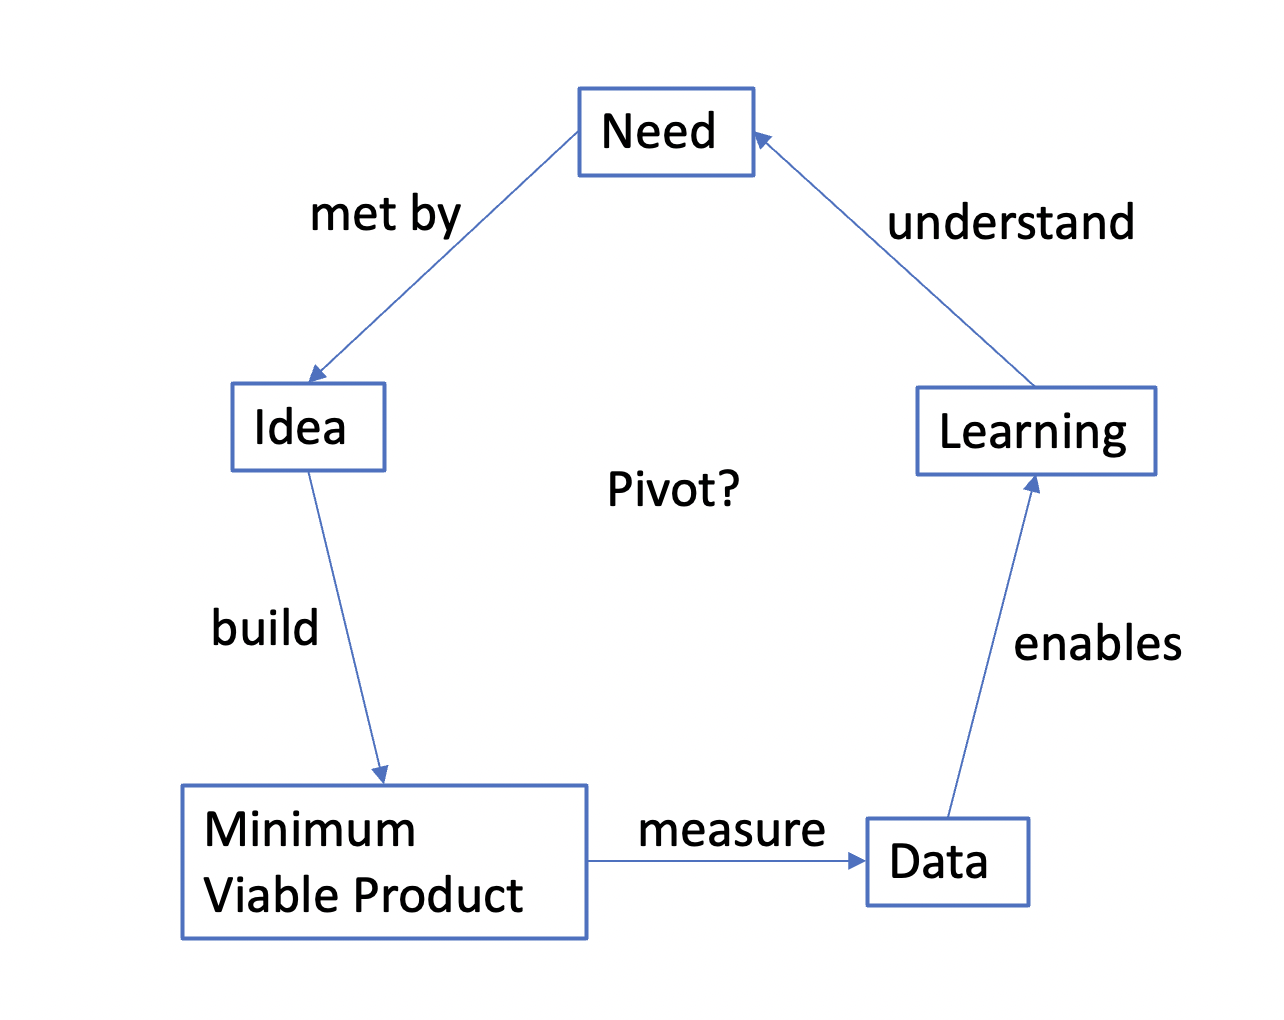
\includegraphics[width=0.8\columnwidth]{Figures/Lean Startup loop}
    \decoRule
    \caption{The Lean Start-up Loop}
    \label{fig:leanloop}
    \end{figure}
    

This loop (\cite{leanstartuploop}), which is shown in \cref{fig:leanloop}, is a depiction of the various potential stages of this project. The current scope of our project covers the 'Need', 'Idea', and 'Minimum Viable Product' stages. These three stages were covered in \cref{marketresearch}, \cref{sec:Introduction} and \cref{sec:UImvp} respectively. \cref{marketresearch} identified potential target customers and their needs. It also highlighted the target customers' likely openness to and acceptance of our digital product. \cref{sec:Introduction} gave a brief outline of this entire design project, which would also introduce the idea we came up with to address our target market needs. \cref{moscow} in \cref{sec:UImvp} gives the specifications for our Minimum Viable Product, which is the actual implementation of our idea. 

For the Data stage, the Minimum Viable Product will be used to gauge consumer response. 
Specifically, we will be testing two hypotheses: the value hypothesis and the growth hypothesis. 
The value hypothesis is a test of whether our product will be delivering any value to customers. 
In other words, we want to check if our product is actually fulfilling its function of converting vocals to chords as well as providing an online platform for a community of amateur musicians. 
We will also want to find out what price customers are willing to pay for our product and its services; specifically, customer response to our subscription-based model outlined in \cref{Source of Cash Inflow}.  
The growth hypothesis is a test of our strategy for acquiring new customers for our product. This is with regard to our tactics such as our marketing, the cost of which will be touched upon briefly in \cref{sec:Finance and Monetisation}. 
While we would collect user feedback, we would also choose objective metrics that will enable informed learning and measure the customers' actual behaviour and not just rely on what they say.

\begin{itemize}
    \item Surveys and interviews (user feedback)
    \item Number of downloads from the App Store
    \item Number of songs for which chords were generated
    \item Number of users (with the number of users who paid for premium services)
    \item Number of posts on the ReChordTogether online platform (with data trends)
    \item Revenue generated from advertisements
    \item Revenue generated from subscription-based model
    \item Number of new users obtained through the refer-a-friend programme
  \end{itemize}

  Gathering all this information will allow us to learn more about our target market, which leads us to the 'Learning' stage. In this stage, we use the data obtained to determine if our initial assumptions about the target market were valid. This leads us back to the 'Need' stage, where we gain a better understanding of the market needs based on what we learned from the data in the previous stage. We can go through this loop multiple times, each time tweaking certain aspects of our product and its services to better serve the customers' needs while maximising profits. In the event our product is not actually feasible, we can pivot to another product or service.

  \subsection{STEEP Drivers}
  \label{STEEP Drivers}

  STEEP is an acronym that summarises the key drivers which can impact a business. It stands for social, technological, economic, environmental, and political. This is a useful tool for predicting possible future market trends.

  \subsubsection{Social}
  There has been a significant shift to digital music making, with the Coronavirus pandemic having accelerated this trend (\cite{abrsm2021}). Furthermore, over one third of parents in the UK report their children taking up an instrument during lockdown, with two thirds reporting their children practising more (\cite{abrsm2021}). Hence, it appears that the pandemic has encouraged the younger generations to take up music. This does suggest that there will be a larger proportion of technology-savvy musicians in the future.

  Interestingly, there may be a trend of consumers becoming less concerned with data privacy. In the UK, the number of respondents to a survey that stated that they were very concerned about the use of their data dropped from 47\% to 24\% (\cite{DeloitteData}). This does mean that we could potentially be able to obtain a larger pool of user data that we can use to fine-tune the machine learning model or to further improve our business model. Of course, we will handle the data legally and ethically as highlighted in \cref{sec:dataethics}.

  \subsubsection{Technological}
  With advancements in the field of machine learning, we will be able to create better models in the future. These models would be better in the sense that they would generate chords that fit the vocals better, resulting in higher user satisfaction. Additionally, future models could be trained to identify the mood of songs solely from the vocals and then generate the mood-appropriate chords instead of having to have users select the mood themselves as in (\cite{MySong}). This idea will be further explored in \cref{Music Mood Classification} and \cref{moscow}.

  Moreover, internet connectivity is projected to increase, from 51\% of the global population being internet users in 2018 to 66\% by 2023 (\cite{cisco_2022}). In fact, 90\% of the projected world population of eight billion are expected to be internet users by 2030 (\cite{cybersecurityventures}). This represents a larger potential user base in the near future.

Machine learning is also increasingly becoming integrated with smartphones, with Deep Learning frameworks such as Core ML from Apple\footnote{https://developer.apple.com/documentation/coreml}, TensorFlow Lite from Google\footnote{https://www.tensorflow.org/lite}, and ncnn from Tencent\footnote{https://github.com/Tencent/ncnn}.
An estimated one third of smartphones shipped in 2020 possessed built-in machine learning capabilities (\cite{counterpointML}). 
Built-in Deep Learning capabilities make user data more secure, allow for continued operation even with poor Internet access, and help mobile application developers to avoid paying for cloud computing (\cite{10.1145/2644865.2541967}) (\cite{https://doi.org/10.48550/arxiv.1704.04861}) (\cite{DL3}) (\cite{7460664}) (\cite{10.1145/2750858.2804262}) (\cite{10.1145/3210240.3210337}) (\cite{10.1145/3241539.3241563}) (\cite{10.1145/3005448}). This is significant given the importance of data privacy as highlighted in \cref{sec:dataethics}, and that almost half of the world has no access to the Internet (\cite{cisco_2022}). Built-in machine learning capabilities also introduce the possibility of more individualised models that is personalised for each user based on their music tastes and preferences. However, as will be discussed in \cref{Sustainability}, cloud computing is more energy efficient than relying on local devices. Hence, it will not be as straightforward as just shifting all computing to local devices and utilising their built-in machine learning capabilities. We will have to balance between our commitment to sustainability and being able to provide more personalised services and offline functionalities to our user base. Nevertheless, this particular technological development is something we will have to pay close attention to in order for our product to gain as much competitive advantage as possible.

\subsubsection{Economic}
There appears to be a shift from record labels to independent artists in the music industry (\cite{worldwide2020}). The amount of money generated by independent musicians jumped 35\% from 2017 to 2018 to reach a total of 643 million USD (\cite{independentartists}). In fact, independent artists are predicted to contribute about 25\% of the total global music industry revenues by 2026 (\cite{rollingstone}). This trend could potentially mean a larger market for our product in the near future.

\subsubsection{Environment}
While this might seem irrelevant to our project, power consumption is actually something that we have to take into account as highlighted in \cref{Sustainability}. Given that more than half of respondents worldwide consider sustainability in consumer choices \cite{GlobalSurvey}, it is prudent to minimise our carbon footprint in order to grow our user base.

\subsubsection{Political}
Government policies have left music education in the UK in a precarious state (\cite{perilousstate}). There have also been funding cuts to music education both on the tertiary and pre-tertiary levels (\cite{weale2021}) (\cite{macdonald2021}). Consequently, music provision in schools have generally declined (\cite{brown2018}) (\cite{weale2018}). Hence, it is reasonable to assume that amateur musicians in the future are more likely to not have in-depth knowledge of music theory and would find the vocal-to-chords functionality provided by our product useful. This potentially represents a larger market that we can capture.
%\subsubsection{Market Research}

%	SECTION 4
%----------------------------------------------------------------------------------------
\tocdata{toc}{Di Wan} 
\section{Risk and Data Security}
\sectionmark{Risk and Data Security - Di Wan}
The two operating systems, the IOS system based on the Apple platform and Android System, that our design was developed on are encrypted by default for data security reasons. Data is ‘sandboxed’ behind a security layer which isolates each app from the operating systems. The app can’t permit itself to access anything, so the permissions system pops up messages asking for access to specific privacy functions such as photos and microphones. That prevents the apps from reading data from other apps or the phone’s operating system unless users give the app permission. It’s on developers to make sure that apps only request the access they need. 
 \\The app developers’ influence over server security can be limited, but we can certainly make recommendations. We attempt to include Transport Layer Security\footnote{Office, C. D. and D. (2021, April 22). Using transport layer security (TLS) in your organisation. GOV.UK. Retrieved May 14, 2022, from https://www.gov.uk/government/publications/email-security-standards/transport-layer-security-tls} in our design, a protocol that encrypts the data and demands that the server and app authenticate before exchanging data. If there’s any problem with the communication between server and app, no data will be exchanged: prevention is better than cure. Beyond that, we will test network security using a Microsoft, and IBM approved SSL tool\footnote{The University of Stanford. (2018, November 28). Vulnerability Management (Qualys). Vulnerability Management (Qualys) | University IT. Retrieved May 14, 2022, from https://uit.stanford.edu/service/qualys } designed by Qualys, which offers a continuous network security assessment and compliance with security standards.
 \\Finding defects in production is expensive, so we need to perform risk analysis during software testing to understand better what can go wrong with an application before it goes into the market. A risk analysis performed during software testing helps identify areas where software flaws could result in severe issues in production. By identifying areas of concern early, developers can proactively remediate and reduce the overall risk of a production defect.

%----------------------------------------------------------------------------------------
%	SECTION 5
%----------------------------------------------------------------------------------------
\tocdata{toc}{Di Wan}
\section{Finance and Monetisation}
\sectionmark{Finance and Monetisation - Di Wan}
\label{sec:Finance and Monetisation}
Our app design project will need a budget to monitor the expenditure throughout the whole development process because a project can fail due to an unexpected shortage of funds. A project budget is the estimated total cost of completing each project activity over each project phase. Based on the statistics published by SPDLoad\footnote{Spdload. (2021, December 28). App Development Cost in 2022 by App Type (\& examples). SpdLoad. Retrieved May 14, 2022, from https://spdload.com/blog/app-development-cost/}, our project will take approximately nine months to finish due to its high complexity, such as machine learning integration and online cooperation.
\subsection{Cost Breakdown}
The cost breakdown is the systematic process of identifying the individual elements that comprise the total cost of a good, service or package. Here we divide our costs into two types: direct and indirect costs.
\subsubsection{Direct Costs}
We define direct costs are the costs proportional to the number of our subscribers, which are costs after our product enters the market in the future.
\begin{itemize}
\item As we currently focus on the IOS design based on the Apple platform and Android design, the biggest two app stores are \textbf{Apple App Store} and \textbf{Google Play}, the retailer charge fee will be 15\% to 30\% depending on the subscription situation\footnote{https://www.theverge.com/21445923/platform-fees-apps-games-business-marketplace-apple-google}. The platform fee can be avoided by redirecting the payment page to our site bypassing the app store platform. However, the extra steps in the payment process introduce more barriers, which may further lead to a more significant fall in the number of subscribers.
\item The average transaction processing fee through card payment will be approximate 2.9\%, based on the statistics published by The Ascent\footnote{Daly, L. (2022, January 13). Average credit card processing fees and costs in 2021: The ascent. The Motley Fool. Retrieved May 15, 2022, from https://www.fool.com/the-ascent/research/average-credit-card-processing-fees-costs-america/}.
\end{itemize}


\subsubsection{Indirect Costs}
We define indirect costs as costs that are not proportional to the number of our subscribers. Those include:
\begin{itemize}
\item \textbf{Labour cost}
\\We will need a team for our app design; based on the post by SPDLoad, a typical app-design team must consist of 1 project manager/product manager (£57,341/ year), 1 UI/UX designer (£39,540/ year), 1 iOS developer (£57,351/ year), 1 Android developer (£53,350/ year), one backend developer (£53,568/ year) and one quality assurance engineer (£44,712/ year), the annual salaries for each team-member is according to average wages in London published by Glassdoor\footnote{Glassdoor job search. (n.d.). Retrieved May 15, 2022, from https://www.glassdoor.com/member/home/index.htm }, which is a website that allows current and former employees to review their company and publish their salary rates.
\item \textbf{Marketing cost}
\\ Marketing costs are all expenses the company makes to market and sell its products and develop and promote its brand. We set our budget to be £10,000.
\item \textbf{Testing cost}
\\ Testing cost is the costs associated with the app testing stage, where we need to employ the service from other companies. The estimate will be £10,000 based on the average app testing cost published by Apphawks\footnote{SunGroup. (n.d.). Breaking down the app testing costs, models, and ways to save. Apphawks. Retrieved May 15, 2022, from https://apphawks.com/blog/breaking-down-the-app-testing-costs }.
\item \textbf{Others}
\\Those are the costs consisting of app development account fees and other utilities. The estimate will be £15,000.
\end{itemize}

Here we present those estimated costs in the table of annual cost sheet (see \cref{costsheet}):

\begin{table}[ht]
\centering
\begin{tabular}{ |c|c|c|} 
 \hline
 &\textbf{Percentage (\%)} &\textbf{ £ Amount }\\
 \hline
\multicolumn{1}{|c}{\textbf{Direct Cost}} &\multicolumn{1}{c}{}&\\
 \hline
 App store retailer fee&$15\%\times N \times P$&\\
 \hline
 Payment transaction fee&$2.3\% \times N \times P$&\\
 \hline
 &&\\
 \hline
 \multicolumn{1}{|c}{}&\multicolumn{1}{c}{}&\\\hline
 \multicolumn{1}{|c}{\textbf{Indirect Cost}} &\multicolumn{1}{c}{}&\\
 \hline
 Labour Costs&&£229,396\\
 \hline
 Marketing&&£10,000\\
 \hline
 Testing&&£10,000\\
 \hline
 Others&&£15,000\\
 \hline
 \multicolumn{1}{|c}{}&\multicolumn{1}{c}{}&\\
 \hline
 \textbf{Total}&\multicolumn{1}{c}{$17.3\%\times N \times P \times M + \pounds 264,396$}&\\
 \hline
 \end{tabular}
 \caption{Annual cost sheet}
 \label{costsheet}
 \end{table}
Where $N$ is number of subscribers, $P$ is the subscription fee per month and $M$ is the number of months. The estimation is based on the assumption that we will hire a whole app project team rather than out-sourcing the whole project to a software company.

\subsection{Source of Cash Inflow}
\label{Source of Cash Inflow}
The source of cash inflow helps maintain the operation of the company.  There are two main sources of cash inflow through our app, advertisements revenue and subscription fee. 
\\ \textbf{Advertisement Revenue}
\\ We have decided to cooperate with other music-related companies and place their advertisements on our app pages; the revenue will be based on the number of clicks. The decision on where we are going to place the advertisement will impact our user experience, further affecting the number of users and revenue. Hence, we will use A/B testing (will be introduced in \cref{ch2test}) to optimise the position for the advertisement and potentially increase advertisement revenue.
\\ \textbf{Subscription}
\\We consider a subscription fee the main source of income for our app, and we aim to provide a monthly subscription model for our users to access the premium functions, such as pitch tracking. We will combine different pricing strategies to determine the price for our subscription features, such as competitive pricing and dynamic pricing. Competitive pricing is about analysing the subscription price of our competitors and setting a price that our app remains competitive. We use dynamic pricing to attract our potential subscribers to try our subscription features by setting a lower price than normal for the first month.

\subsection{Estimation}
The leading apps we are competing with are Chordify, Chord AI and MySong (\cite{MySong}). Although MySong is a chord generation system, since it is only limited to educational use we will not consider it as our competitor. All the primary functions of these apps and our app are to generate chords to accompany a melody.  Therefore, it is reasonable to estimate the user size of our app based on $max[\text{user size of Chordify, user size of Chord AI}]$. However, there is no public data that reveals the user sizes of these two apps. We finally estimate our potential user size by adding the number of reviewers of Chordify and Chord ai and scaling the total number by 2, which is an approximation of assuming 50\% users gave reviews for apps, based on the statistics published by GlobalWebIndex\footnote{Commerce - GlobalWebIndex. (n.d.). Retrieved May 15, 2022, from https://www.gwi.com/hubfs/Downloads/Commerce\_Report.pdf}. Hence, we estimate our potential user size to be around 80,000. If we assume our app is well accepted in the future by our users and 50\% of them are willing to subscribe to our premium features for the whole year, we can calculate the minimum price we should set for our subscription feature to be £0.67 per month by equalling cost to the revenue. The estimated price is quite competitive compared to the subscription fees of Chordify (£1.24/month) and Chord AI (£3.49/month).
%----------------------------------------------------------------------------------------
%	SECTION 6
%----------------------------------------------------------------------------------------
\tocdata{toc}{Kitty Fung}
\section{Ethics}
\sectionmark{Ethics - Kitty Fung}
\label{sec:dataethics}
From the National Society of Professional Engineers Code of Ethics (\cite{codeofethics}), it is of the utmost 
importance to ensure engineering work upholds honesty, impartiality, fairness, and equity, and must be dedicated to 
the protection of the public health, safety, and welfare. Since our design interacts with users
through a mobile application, ethical concerns have arisen regarding the interactions between users 
and data handling on our end. In this section, we will address issues related to data ethics.

Governmental organisations have published regulations (\cite{EUdataregulations2018}) and frameworks
(\cite{framework}) that are minimum standards for handling data ethically. The core value of data ethics 
is to treat data responsibly and righteously.

There are three overarching principles to adhere to, but in short, we as the developer should treat our 
users\textsc{\char13} data as we would for our own.

\subsection{Transparency}
We should be clear and publish specifications of our project in a way that users can understand and access
easily. It is necessary to delineate a privacy policy to make sure users read and agree to it before they use
our application and keep the policy at a prominent location, i.e. in the footer for the webpage, in the developer
section of the app listing or on the sign-in interface of the app.\\We would include the following items in our privacy policy:
\begin{enumerate}
    \item \textbf{Company licence and registration reference number:} Registration at the Information Commissioner's Office is required
    before collecting data from the public.
    \item \textbf{Details and purpose of data collected:} We should limit data collection to what is necessary and to an explicit goal.
    Thus, we will collect:
    \begin{description}
        \item[Personal details -] Name and email address are the necessary fields. Gender, age and profile picture are optional inputs 
        that will help improve the user experience and accuracy of the model. 
        \item[Audio data -] Audio signal and metadata to feed into our machine learning model to improve accuracy.
        \item[Networks and connections -] Collected for our interactive community features.
        \item[Usage -] Contents and functions that the users have viewed or engaged with and the duration.
        \item[Device information -] Device attributes like signal strength, battery levels, and operating system version to adjust our app's operation.
        \item[Cookie data -] Both first- and third-party cookies are needed. For first-party cookies, to personalise and optimise user
        experience, we would save their usage preferences like language, and dark or light background mode. 
        \\There are two purposes for using third-party cookies. Firstly, since we will be displaying advertisements, 
        these advertising companies will be able to place cookies on our app for standard users, but not the premium users who subscribed to our services. 
        Secondly, we will be implementing social sign-on, so users do not have to create a new account on our end. In this case, the social media 
        platform will be placing its third-party cookies on our app.
        \\It is important to note that users have the right to know the third parties that have access to their data.
    \end{description}
    \item \textbf{Data retention policy:} We will specify how long information will be kept and the procedure of disposing of the data when a user deactivates
    his account or when the data is no longer necessary to collect. Moreover, we would have to erase or rectify inaccurate data without delay. Although 
    there is no limitation on data storage, we will have to act ethically and
    decide the timeframe based on the genuine motivation of retaining the data. Data should only be collected when it is vital in the context
    of app operation. Thus, we should not keep data just in case it is needed in the future. For data that has expired (past the retention period), we 
    would have to either delete it or anonymise it. If we are to delete the data, we have to ensure all digital and hard copies of the data are destroyed. 
    This action requires careful documentation of data storage from the date we collect data from users, as traces may often reside in forgotten databases.
    Anonymising data means that a piece of information cannot be associated with an identity, which will not help with improving user experience, but still 
    can be used to monitor the entire application performance.
    \item \textbf{Access rights within the team:} Different team members of our project will have access rights to different types of data collected from
    the users, and we should delineate who will be responsible for which part of the data we store.
    \item \textbf{Rights that users have over their data:} Users should have the right to request a copy of data provided, request us to delete the data and object to our data processing.
    \item \textbf{Notification of changes to privacy policy:} We will contact users to review and accept the revised policy through email.
    \item \textbf{Security standards:} We should specify the encryption standards and the processes in place to test the confidentiality, integrity and availability of 
    our system.
    \item \textbf{Contact information:} Contact details like organisation contact number, email address, office and postal address.
\end{enumerate}

\subsection{Accountability} 
We should process personal data responsibly and systematically, as well as endeavour to reduce risks for individuals and mitigate social and ethical implications (\cite{principles}).
This can be done by creating a department that overviews the entire project and ensures data is managed ethically throughout the process. As we have an interactive community 
feature, we must ensure that our app does no harm in any way. A new Online Safety Bill is being drafted recently to fight online hate crime, and online companies are liable for failures to
deal with inappropriate material posted online (\cite{francis}), (\cite{parliamentlaw}). Companies have the responsibility to confine illegal and harmful discussions, and a conventional and efficient method
to guarantee this is to implement algorithmic censorship. 
Moreover, effective governance and oversight mechanisms that the public can exercise are necessary to be publicly accountable. 
We can enact this by hiring an independent third-party audit to review our data processing.

\subsection{Fairness}
We should ensure no societal, racial or health bias is involved when processing data. Our project collects minimal personal data, so the problem of differential processing for distinct groups can be avoided. 
On the other hand, another perspective of fairness can be manifested in the form of \textbf{Responsible Research and Innovation (RRI)}, which is a process that seeks to promote creativity and opportunities 
for science and innovation that are socially desirable and undertaken in the public interest (\cite{ukri}). Not only does research bring novelty 
and value to society, it may also bring forward ethical dilemmas, social transformations and adverse consequences for society. Thus, it is key to emphasise innovating responsibly and creating changes that
have positive societal and environmental impacts.\\ There are a few areas of RRI that we should keep in mind:
\begin{enumerate}
    \item Anticipation: We should envision the consequences of our research and innovation. It ensures that the research design considers and reflects the effects of undertaking the research. Although we are not creating physical technology in this project, we are building a platform that allows users to communicate with each other. Our app may become a breeding 
        ground for an online hate crime if not dealt with carefully.
    \item Reflection: researchers should always reflect on the research question they are investigating, the type of data collected, the method used to analyse the data and the implications.
    They should also judge if the research is required. An organisation can reflect through organisational processes and structures like a project advisory board or quality assurance reviews. Reflection 
    allows researchers to review the project from a macroscopic point of view.
    \item Ethics: Researchers should uphold the integrity and prevent misconduct. They should take accountability for both the undergoing research and behaviour.
    \item Gender Equality: Since male engineers still dominate the engineering industry, it is easy to be biased in a project design, i.e. building models and interfaces that better suit male users. Thus, it is 
    paramount to have opinions from the underrepresented group to create a comprehensive innovation.
    \item Open Access: Making the research output publicly available to everyone, so the whole society can benefit by reducing wasteful duplication and increasing transparency and reproducibility of results.
    \item Governance: Organisations should establish practices that foster RRI, i.e. 
    \begin{itemize}
        \item Having transparent and reflective internal procedures
        \item Promoting participatory governance
        \item Fostering stakeholder engagement exercises
        \item Encouraging future-oriented governance
        \item Valuing responsiveness
    \end{itemize}
    \item Public Engagement: Researchers should settle upon motivation and the right audience before any public engagement. For our project, the goal would be to allow amateurs to enjoy composing music without
    music professionalism.
\end{enumerate}
%----------------------------------------------------------------------------------------
%	SECTION 7
%----------------------------------------------------------------------------------------
\tocdata{toc}{Kitty Fung}
\section{Sustainability}
\sectionmark{Sustainability - Kitty Fung}
\label{Sustainability}
As technology advances, energy consumed by computers and personal digital devices is taking up a more significant portion of worldwide energy consumption. 
According to an article published by \citebracks{energypy} and a research done by GO-Globe (\cite{energy}), there are about 8,918,157,500 active
mobile devices consume a total of $3.46\times 10^{12}$ kWh energy per year.
While a lot of effort has been put into reducing the energy consumption from the hardware perspective,
it is also prime to focus on the impact of software implementation.
Other than writing energy-efficient codes (i.e. optimised searching and sorting algorithms), the programming language 
chosen can make a substantial difference too. Energy, time and memory size are the significant resources required for running a program.
At first glance, since \(Energy = Power * Time\), there seems to be a correlation between energy and time. Yet,
\citebracks{energyplanguage} suggests that since \(Power\) is not a constant, we cannot draw the conclusion that
when \(Time\) increases, \(Energy\) must increase. 
Pereira ranked the performance of different programming languages according to their energy, time and memory size consumption (p.7). 
Surprisingly, there is no strong correlation between these three components. 
Instead, the performance depends on the category of the programming language.
The programming languages can be divided into three execution types: compiler, interpreter and virtual machine.

\begin{description}
    \item Compiler converts the entire high-level language code to machine-readable language. Some examples are C, C++, Rust and Go. 
    \item Interpreter translates one statement of the high-level language code to machine-readable language at a time. Common interpreted languages are PHP, Python and JavaScript.
    Thus, even if an interpreter takes less time to analyse the source code, it takes longer to execute the process.
    \item Virtual machine executes an intermediate code translated from the high-level language inputted. Some popular languages that use virtual machines are Java, Scala, and JRuby.
\end{description}

Since our application has no computational time and memory size requirements, we can solely focus on the energy consumption between 
different languages. Even though the energy needed to run various algorithms varies for other languages, it is inevitable that
compiled language requires less energy compared to the virtual machine and interpreted languages. Our team has used Python for the design and implementation, so 
it is rational to switch from Python to C/ C++/ Rust to code in the future.

We can reduce energy consumption by 87\% by employing a cloud architecture (\cite{cloudpercent}).
Yet, researchers have shown that cloud computing is more energy-efficient than relying on local devices (i.e. using our private data centres, computing on
users\textsc{\char13} smartphones).

Firstly, taking Amazon Web Services (AWS), the leading service provider in the cloud infrastructure market, as an example, it aims to fully power the operation with renewable
energy by 2025 \citebracks{aws}. Since it is complex and cost-ineffective for individuals or small-scale companies to switch to clean energy, using the cloud services provided
by eco-conscious companies would significantly reduce their carbon footprints.

On the other hand, a centralised cloud provider allocates resources more efficiently since there is a higher utilisation rate. If we choose an on-premise computing method, we will suffer
from low utilisation rates since the purchased equipment may only be fully utilised when there are usage spikes. Yet, cloud providers have a vast customer base, and it is paramount for 
their businesses to optimise server usage. Thus sharing cloud servers can increase average server utilisation to 50 per cent or higher (\cite{cloud}).

% Therefore, we should carefully design our architecture and minimise carbon footprints.